\FloatBarrier
\subsubsection{Detection system}\label{sec:detection}
%\emph{Author(s): S.\ Hild and R. Goauty \\}
Traditionally detection system of first and second generation gravitational wave detector includes all
optical elements downstream the main interferometer (i.e. behind the signal
recycling mirror), such as for instance the readout photodiodes and the output mode
cleaner (OMC). In contrast,  as described already described in section~\ref{subsec:QNRsqz}
ET will feature the injection of frequency dependent squeezed light from the back of the interferometer
and there are lots of hardware components required for this purpose, such as for instance the squeezed light sources
as well as the filter cavities. In this section we will focus on the traditional components of a the detection
subsystem, i.e. the readout of the main gravitational wave signal and the output mode cleaner. 

\FloatBarrier
\paragraph{Readout options for the gravitational wave signal}

\begin{figure}[th]
\centering
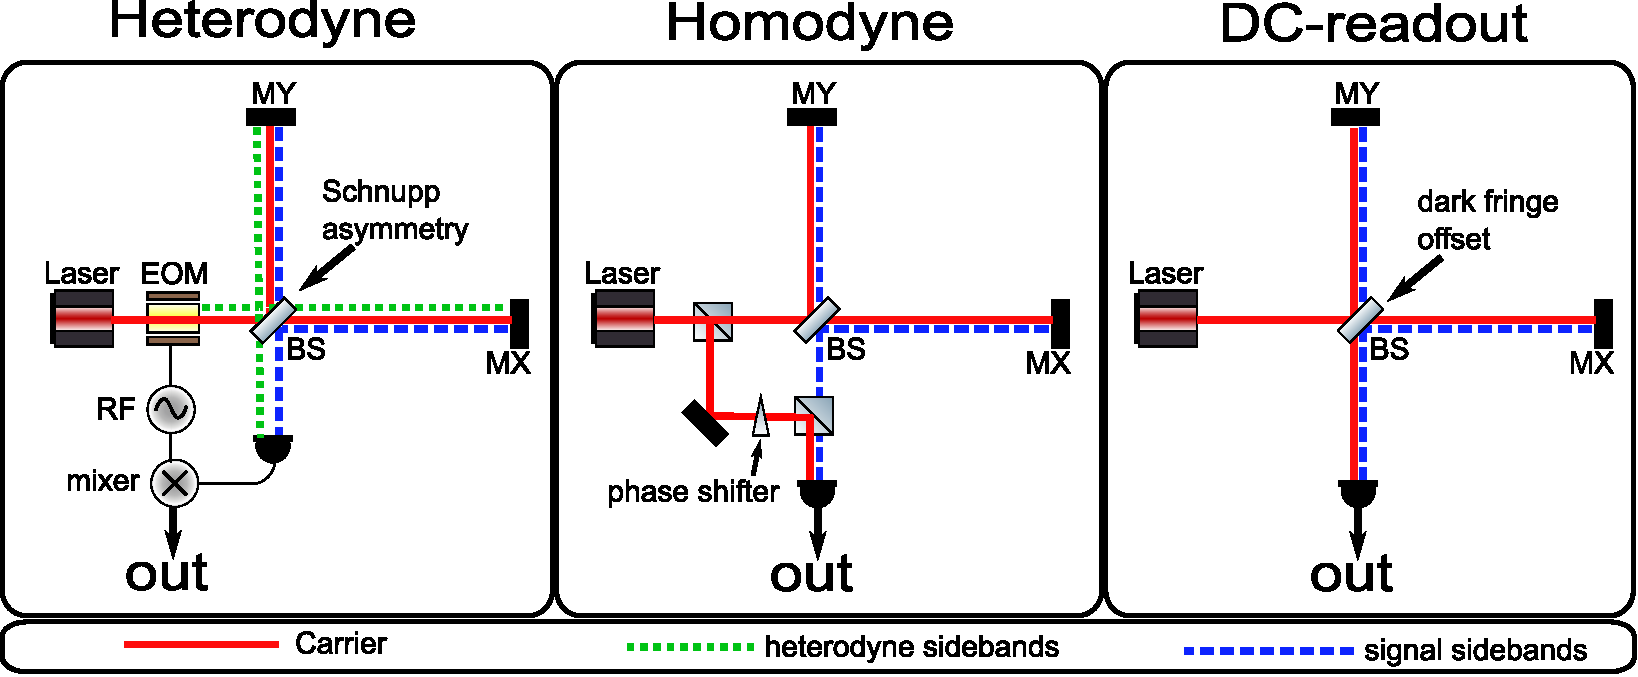
\includegraphics[width=1\textwidth]{Sec_Optics/homo_hetero_schematic.pdf}
\caption[Different readout methods of a Michelson interferometer]{Illustration of three different 
readout methods of a Michelson interferometer:
heterodyne, homodyne and DC-readout. A detailed explanation is given in the text.}
\label{fig:principle}
\end{figure}


Figure~\ref{fig:principle} shows simplified schematics of three different readout
methods applied to a basic Michelson interferometer. Usually Michelson
interferometers used for gravitational wave detection are operated at the dark
 fringe, which  has the advantage
 of providing good suppression of common mode noise and allows to 
make use of power recycling.
The differential arm-length is controlled
to give destructive interference at the output port: ideally
 no carrier light ($f_{\rm c}$, red solid line) reaches the photo detector.
 A change of the differential arm length causes phase modulation
sidebands, i.e. gravitational
wave signal sidebands (blue dashed line). In contrast to the carrier light the gravitational
wave signal sidebands
 interfere constructively at the beam splitter, exit the interferometer towards its output port
and finally reach the photo detector.
The absolute frequency of the gravitational signal sidebands is given
 by $f_{\rm sig} =  f_{\rm c} \pm f_{\rm gw}$, where $f_{\rm gw}$ is the
 frequency of the gravitational wave (usually in the audio-band) and $f_{\rm c}$ 
the frequency of the main laser light (carrier).
Since $f_{\rm sig}$ is
a few hundred terahertz, the photodiode cannot directly detect
the gravitational wave signal, unless the presence of an optical local oscillator
is ensured. Heterodyne, homodyne and DC-readout are three different concepts to
ensure the presence of a low-noise optical local oscillator at the output port photodiode.


In the heterodyne scheme, commonly used by the first generation
gravitational wave detectors,
 radio frequency  sidebands ($f_{\rm het}$, green dotted lines)
are modulated onto the light at the input of
the Michelson interferometer (Schnupp modulation \cite{Schnupp1988}).
Introducing a macroscopic arm length difference of several centimeter
 (so-called Schnupp asymmetry) allows the modulation
sidebands to be transferred through the interferometer to the output port,
where they serve as optical local oscillator for the differential arm length  signal.
The photo-current produced by the beat between the different optical
field components (optical demodulation) contains
a radio frequency component at $f_{\rm het} \pm f_{\rm gw}$. In a second demodulation
process the photo-current is then electronically demodulated at $f_{\rm het}$ 
 in order to finally derive a signal stream at $f_{\rm gw}$.


In the homodyne readout scheme (center plot of Figure~\ref{fig:principle}) a  small
fraction of the carrier light is split off in front of the interferometer and guided directly
to the output photo detector without passing through the interferometer.
The big
advantage of this form of homodyne readout is that a phase shifter,
 placed in the local oscillator path, allows an easy
change of the optical demodulation phase, i.e.\ the readout quadrature,
without any hardware changes. On the other hand homodyne
readout has the disadvantage that the length and the alignment of the local-oscillator path needs to be highly stable.
In practice this usually implies that the local-oscillator path length as well as its alignment need to be actively
stabilized by a low-noise control system, and all components of the local-oscillator path must be
 seismically isolated inside a vacuum system.
Due to these demanding noise and hardware requirements, so far there have
been no serious plans to change
the readout scheme of the currently operating gravitational wave detectors
from heterodyne to homodyne readout.


DC-readout is a special case of homodyne readout which
is much easier to combine with the existing elements of  currently used
gravitational wave detectors.
In a DC-readout  scheme the operating point of the Michelson interferometer is slightly
shifted off the dark fringe, by introducing a so-called \emph{dark-fringe offset},
thus a certain amount of carrier light leaves the interferometer at the output port
 and can serve as local oscillator. Compared with the previously described homodyne readout,
DC-readout has the advantage that no additional local oscillator path outside the main interferometer
is required. On the other hand, DC-readout offers no easy way to vary the phase of the
optical demodulation.

DC-readout was already used in the first `Michelson' interferometer ever by Michelson and Morley
in 1887~\cite{michelson1887}. It is probably the simplest way to read out a Michelson
interferometer, but was considered to be unsuitable for the first generation of gravitational
wave detectors due to the strong coupling of laser power noise. However, increased
stability of the laser power inside future instruments gives hope for a renaissance
of DC-readout for gravitational wave detectors, which was first proposed
by Fritschel~\cite{Fritschel2}. 

The next section briefly summarises the general advantages and disadvantages of
DC-readout compared with heterodyne readout, especially taking into account the implications
for an interferometer with tuned or detuned signal recycling \cite{Hildtuned_detuned2007}.

\FloatBarrier

\etbox{i}{ibox:DC-readout}{Motivation for using DC-readout in ET}
{
DC-readout has several advantages over heterodyne
readout:
\begin{enumerate}
\item
DC-readout provides an increased 
signal to shot noise ratio compared to heterodyne readout \cite{Buonanno2003}. This is 
due to the fact that in the homodyne detection the shot noise contribution from frequencies 
twice the heterodyne frequency 
does not exist. 
\item
In DC-readout a reduced number of beating light fields at the detection port potentially reduces and 
simplifies the cross-couplings of technical noise \cite{Hildtuned_detuned2007}. Especially 
the coupling of amplitude and phase noise of the heterodyne modulation is 
strongly reduced in a DC-readout scheme. 
%\item
\item
A simpler calibration procedure can be applied for DC-readout, because the GW-signal is present in a single
data-stream even for
detuned signal-recycling (and not spread over the two heterodyne quadratures as
described in~\cite{Hewitson05}).
\item
As with DC-readout the main photodiode(s) and electronics for the detection do not need to be capable of
handling RF signals, they can be simplified.
\item
Large-area photodiodes may be used in DC-readout. These should offer reduced coupling of beam-pointing 
noise, due to decreased beam clipping and decreased influence of 
photo diode inhomogeneity (by averaging over a larger area). 
\item
As in the DC-readout configuration the local oscillator and the GW-signal pass the same optical system an 
optimal spatial overlap is guaranteed. (Due to thermal distortion current GW detectors 
employing arm cavities encountered the problem of imperfect spatial overlap of the carrier light 
(GW signal) and the heterodyne sidebands (local oscillator) \cite{Lawrence03})
\item Finally, the realization of a squeezed light enhanced
interferometer is simpler using DC-readout rather than heterodyne
readout. DC-readout requires squeezed light to be present only at
frequencies in the GW signal bandwidth compared to heterodyne
readout which requires squeezed light around twice the heterodyne
frequency as well~\cite{CDRGBM98}.
%\footnote{A squeezed light
%source working only in the GW signal bandwidth would result in the
%DC-readout case in a sensitivity enhancement limited by the squeezing
%strength generated, whereas the same source would act in a
%heterodyne-readout based interferometer as if 50\% of the squeezing
%was reduced due to losses. Hence, a sensitivity improvement by a
%factor of 6\,dB in the DC-readout case would result in the heterodyne
%case in an improvement factor of only 2\,dB.}
\end{enumerate}
}
%
This long list of advantages has to be compared with the drawbacks of DC-readout.
Even though power fluctuations of the carrier light (i.e. the local oscillator) 
are strongly filtered by the cavity poles of the power recycling cavity and the 
high-finesse arm cavities, the major disadvantage of DC-readout is  an
increased coupling of laser power noise. For the Einstein Telescope the advantages
of DC-readout clearly way out the disadvantages and therefore DC-readout was chosen as 
baseline configuration for the gravitational wave readout.


Recently enhanced LIGO and GEO-HF have successfully demonstrated the application
of DC-readout in long-baseline gravitational wave detectors. Furthermore, all advanced 
gravitational wave detectors plan to use DC-readout for the gravitational wave 
signal. Therefore, the commissioning of Advanced LIGO and Advanced Virgo is expected to greatly inform 
the technical design of the ET readout system. 

\FloatBarrier

\paragraph{Output mode cleaner}

The beam transmitted at the output port of each interferometer must be filtered by an Output Mode Cleaner cavity (OMC). 
The goal of the OMC is to filter the imperfections of the beam profile that are induced by beam mismatch, misalignment
 or astigmatism defects in the interferometer. Such defects couple a fraction of the main beam into spurious geometrical
  modes which do not carry information on differential arm motion. Therefore, by eliminating these spurious modes before 
  the beam reaches the photodiodes, the OMC plays a crucial role in minimizing the shot noise.

For a DC-readout interferometer, only the carrier component of the beam is involved in the detection of a gravitational wave
 signal. On the other hand, modulation sidebands which are used for longitudinal and angular sensing in the mirror control 
 loops do not play any role for detection. Therefore, the OMC should suppress the modulation side bands in order to minimize 
 the shot noise and also to prevent the side band power noise from spoiling the sensitivity.
The main parameters to be defined for the OMC are: the geometry and the type of the cavity, the finesse, the length and
 the waist.

The favored geometry is a bow-tie cavity made of four reflective surfaces as shown in Figure~\ref{fig:sc_geometry}. 
Two of these surfaces are curved in order to introduce a Gouy phase between different geometrical modes. Such cavity is 
compatible with the Laguerre-Gauss High Order mode technology, and would be suitable for both the ET-LF (TEM$_{00}$ beam) 
and ET-HF (LG$_{33}$ beam) instruments. A bow-tie cavity also allows a small incidence angle between the beam and the OMC 
surfaces. One can envision an incidence angle of the order of 10 degrees as it is foreseen for Advanced Virgo. This choice should 
make it possible to minimize the amount of back-scattered light without introducing too much astigmatism.

Two types of cavity can be envisioned: a monolithic cavity made of a few centimeters long crystal as it has been designed for Advanced
 Virgo~(\cite{VIR-NOT-071A-08} and \cite{VIR-0020A-11}) or a `tombstone' design as for Advanced LIGO~\cite{LIGO-T1000276} or GEO600~\cite{Degallaix10, Prijatelj10}. The tombstone 
 OMC consists of four individual mirrors rigidly connected by a spacer and whose round-trip length can be of the order of 1\,m. The main
  advantages and drawbacks of these designs are discussed below.

The monolithic design is a robust and compact solution that already benefits from a long and successful experience with the Virgo OMC. 
A monolithic OMC can be kept at resonance using a thermal length control based on a Peltier as actuator. The error signal can be obtained by 
modulating the OMC length using a small PZT actuator placed on top of the cavity. As it has been proven with the Virgo OMC, this 
system can be arranged so that its mechanical resonances lie well above the detector bandwidth~\cite{Derome97}. Thus this device is 
very stable from a mechanical point of view. Another big advantage is a low thermal noise, which is an important criterion as OMC 
length fluctuations can spoil the sensitivity. A recent measurement with the Virgo interferometer was used to put an upper limit on the 
OMC length fluctuations due to thermal noise of $6 \times 10^{-17}~{\rm m}/\sqrt{\rm Hz}$ at $100$\,Hz~\cite{VIR-0020A-11}. 
%Such upper limit matches
% or is close to match the requirements for ET with an assumed finesse of $260$ and a OMC locking accuracy of $10^{-12}~m$. 
 The main weakness of the monolithic design is the limitation on the length which cannot be increased too much in order to keep 
 the thermal control simple and the mechanics stable. As the OMC length has a direct impact on the filtering performances of spurious 
 geometrical modes and side bands, this criterion will have to be examined very carefully before making a final choice on the type of 
 cavity. Another potential weakness of a monolithic OMC is the risk of thermal effects due to absorption of the laser power in the OMC
  substrate and thermal lensing. This risk becomes higher with the ET-HF instrument for which the power reaching the OMC should be 
  four times larger than the expected power for Advanced Virgo. The characterization of thermal effects with the Advanced Virgo OMC
   will be very valuable to better assess this risk.

The tombstone design has been implemented in the Enhanced LIGO~\cite{LIGO-T1000276} and the GEO\,600~\cite{Degallaix10, Prijatelj10} 
interferometers. It is also being designed for the Advanced LIGO project~\cite{LIGO-T1000276}. The main advantage of the tombstone 
design is the absence of strong limitation on the cavity length, which could be of the order of 1\,m. This offers stronger filtering 
performances with respect to a few centimeters long monolithic crystal of equal finesse. Also with this design there should be no
 risk associated to thermal effects due to the high laser power in ET-HF. The OMC length can be controlled by acting on the mirror 
 positions with PZT actuators. Such actuators have a larger bandwidth but are likely to be noisier than the thermal control implemented 
 for the Virgo monolithic OMC. The main weakness of the tombstone design is its higher mechanical complexity. For instance the
  enhanced LIGO detector has experienced some difficulties with the locking of its tombstone OMC. A more reliable actuation system is 
  needed for ET. OMC mechanical resonances have been observed in the detection bandwidth of the  enhanced LIGO and GEO\,600 detectors.
   For the ET design mechanical resonances should be shifted to higher frequencies in order to not spoil the sensitivity. Moreover the
    length noise of such cavity could represent a risk that will be better assessed with the experience of GEO-HF and Advanced LIGO.

The choice between the monolithic or tombstone design will thus result from a trade-off between a conservative filtering of the side 
bands and a low length noise.
The choice of the OMC finesse and length is driven by the filtering needed for the side bands. The main constraints on the filtering 
will be imposed by the sideband power noise which can limit the sensitivity if modulation sidebands are not sufficiently well suppressed. 
Keeping a similar design as for the Advanced Virgo OMC will lead to rather hard constraints on this noise: the relative intensity noise 
of the oscillator signal delivered by the generator should be kept below $10^{-8}~{\rm Hz}^{-1/2}$ at 10\,Hz for ET-LF, and in the range 
$10^{-9}-10^{-8}~{\rm Hz}^{-1/2}$ at $100~{\rm Hz}$ for ET-HF. These specifications seem to be quite challenging. The experience that will be 
gained with Advanced Virgo and Advanced LIGO will help understanding if they are achievable. In case the specifications on the side 
band power noise need to be relaxed, the finesse or length of the OMC cavity should be increased.

The choice of the finesse is limited by the amount of diffraction losses on the OMC mirrors. Assuming losses of the order of $30~ppm$ 
per face, one would need to choose a finesse below $260$ in order to keep the total losses below $1\%$. A better evaluation of the 
expected diffraction losses on the OMC surfaces is needed to assess the limitation on the finesse.

The OMC radius of curvature will be chosen in order to sufficiently filter the spurious geometrical modes of the carrier and side bands. 
Its final choice will depend on the modulation frequencies selected for longitudinal and angular sensing.
In order to prevent laser frequency noise to couple through the OMC, the main laser of ET-LF and ET-HF should be stabilized at low 
frequency using a rigid cavity.

The OMC needs to be associated to several other optical components. In order to limit the amount of back-scattered light a Faraday 
Isolator should be placed in front of the OMC. A telescope should be designed in order to tune with sufficient accuracy the beam matching
 and the beam alignment with respect to the OMC. The whole system should be seismically isolated and placed under vacuum in order to
  meet specifications on beam jitter~\cite{VIR-0054A-11}.
  
  